\chapter{Nonlinear state estimation} \label{ch:nls}
This chapter will introduce a powerful framework for nonlinear state estimation based on nonlinear least squares.
This includes a simple notation for expressing such problems, and a procedure for obtaining the MAP estimate and its uncertainty, given Gaussian measurement noise.
Most of this chapter is based on \cite{Dellaert2017, barfoot2017state}.

\section{Linear least squares}
Consider a set of $n$ \emph{linear} equations in $m$ unknowns $\vecx = [x_1, \ldots, x_m]\trans$
\begin{equation}
  e_i(\vecx) = 0, \quad i = 1, \ldots, n.
\end{equation}
We can combine these equations on vector form as
\begin{equation} \label{eq:ls-equations}
  e(\vecx) = 
  \begin{bmatrix}
    e_1(\vecx)\\
    \vdots\\
    e_n(\vecx)
  \end{bmatrix}
  = \matr{0},
\end{equation}
where $e: \bbR^m \to \bbR^n$.

When $n > m$, it is typically not possible to find an exact solution to \eqref{eq:ls-equations}.
We can instead seek a solution that minimises the sum of squares of the \emph{residuals} $e(\vecx)$,
\begin{equation}
  f(\vecx) = e(\vecx)\trans e(\vecx) = \norm{e(\vecx)}^2,
\end{equation}
where $f(\vecx)$ is often called the \emph{objective function}.
Since \eqref{eq:ls-equations} is linear, we can obtain an objective function on the form
\begin{equation} \label{eq:objective-form}
  f(\vecx) = \norm{e(\vecx)}^2 = \norm{\matA\vecx - \vecb}^2,
\end{equation}
which means that we want to find the vector $\vecx$ so that
\begin{equation} \label{eq:ls-min-residual}
  \vecx^\ast = \argmin_\vecx f(\vecx) = \argmin_\vecx \norm{\matA\vecx - \vecb}^2.
\end{equation}
This is called a \emph{linear least squares} problem.

A solution to \eqref{eq:ls-min-residual} is required to have zero gradient, so that
\begin{equation}
  \dpar{f(\vecx^\ast)}{\vecx^\ast} = 2 \matA\trans (\matA \vecx^\ast - \vecb) = \matr{0}.
\end{equation}
This results in \emph{the normal equations}
\begin{align}
  \matA\trans \matA \vecx^\ast &= \matA\trans \vecb \label{eq:ls-normal-equations}\\
  \vecx^\ast &= (\matA\trans \matA)^{-1} \matA\trans \vecb,
\end{align}
which can be solved with Cholesky- or QR factorisation\footnotemark.
\footnotetext{Equivalent to \texttt{x = A\textbackslash b} in Matlab.}

\section{Nonlinear least squares}
When the equations in $e(\vecx)$ are nonlinear, we have a \emph{nonlinear least squares} problem.
This results in a nonlinear objective function, which cannot be minimised directly using the normal equations in \eqref{eq:ls-normal-equations}.
We can instead assume that $f(\vecx)$ is approximately linear locally around the current estimate.
This lets us define a procedure starting from a suitable initial estimate, where we iteratively linearise the problem, solve the linearised problem using the normal equations, and update the estimate until convergence (Figure~\ref{fig:nls-procedure}).
\begin{figure}[htb]
    \centering
    \tikzstyle{process} = [rectangle, minimum width=9cm, minimum height=1cm, text centered]
\tikzstyle{arrow} = [ultra thick,->,>=stealth]

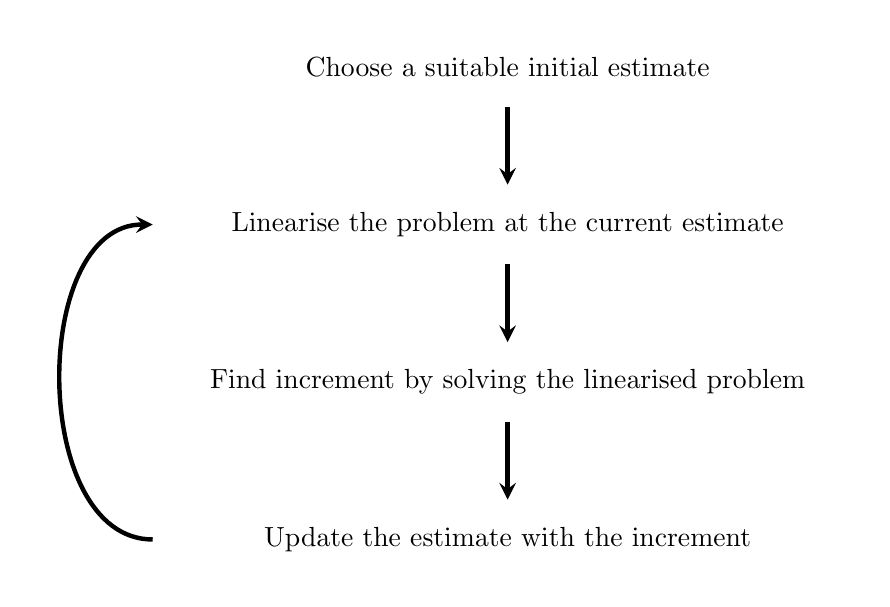
\begin{tikzpicture}[node distance=2cm]
\node (init) [process] {Choose a suitable initial estimate};
\node (linearise) [process, below of=init] {Linearise the problem at the current estimate};
\node (solve) [process, below of=linearise] {Find increment by solving the linearised problem};
\node (update) [process, below of=solve] {Update the estimate with the increment};

\draw [arrow] (init) -- (linearise);
\draw [arrow] (linearise) -- (solve);
\draw [arrow] (solve) -- (update);
\draw [arrow] (update.west) to [out=180,in=180] (linearise.west);
\end{tikzpicture}
    \caption{An iterative procedure for solving nonlinear least squares problems.}
    \label{fig:nls-procedure}
\end{figure}

The vector $\vecx$ is sometimes called a \emph{state variable}, which is typically used to describe the physical state of an object or a system.
The pose of a camera in the world is an example of such a state variable.
Notice that we can concatenate several different state variables into the vector $\vecx$, 
\begin{equation}
  \vecx = 
  \begin{bmatrix}
    \vecx_1\\
    \vdots\\
    \vecx_p
  \end{bmatrix},
\end{equation}
and that the equations $e_i(\vecx)$ can be defined to operate on one or more of these $p$ different state variables.
This lets us use the least squares framework to estimate several state variables at once, such as the poses of a whole set of cameras, instead of only one.

To conveniently represent state variables over both vector spaces and manifolds, we will broaden the definition of the plus and minus operators given in Section~\ref{sec:lie-plus-and-minus}.
First, the vectors $\vecx \in \bbR^m$ is a Lie group under addition, where the exponential map is the identity \cite{SolaARobotics}:
\begin{equation}
  \Exp: \bbR^m \to \bbR^m; \quad\quad \vecx = \Exp(\vecx).
\end{equation}
This means that $\vecx$ is its own tangent vector, and that $\oplus$ and $\ominus$ are in fact valid representations of vector addition and subtraction:
\begin{align}
  \vecx_a \oplus \vecx_b &= \vecx_a + \vecx_b\\
  \vecx_b \ominus \vecx_a &= \vecx_b - \vecx_a,
\end{align}
where $\vecx_a, \vecx_b \in \bbR^m$.

We can now define $\ubar{\cX}$ as the concatenation of state variables
\begin{equation} \label{eq:concatenated-states}
  \ubar{\cX} \triangleq
  \begin{Bmatrix}
    \cX_1\\
    \vdots\\
    \cX_p
  \end{Bmatrix}
  \in \cM,
\end{equation}
where $\cX_i \in \cM_i$ and $\cM = \{\cM_1, \ldots, \cM_p\}$ is the \emph{composite manifold}, which can cover both vector spaces, orientations, poses and other manifolds.
We define $\ubar{\vectau}$ to be the corresponding concatenation of tangent vectors
\begin{equation}
  \ubar{\vectau} \triangleq
  \begin{bmatrix}
    \vectau_1\\
    \vdots\\
    \vectau_p
  \end{bmatrix}
  \in \bbR^m,
\end{equation}
where $\vectau_i$ is in the tangent space of $\cM_i$.
This lets us define the plus and minus operators for the concatenated state variable $\ubar{\cX}$ as
\begin{align}
  \ubar{\cX} \oplus \ubar{\vectau} &\triangleq
  \begin{Bmatrix}
    \cX_1 \oplus \vectau_1\\
    \vdots\\
    \cX_p \oplus \vectau_p
  \end{Bmatrix} \in \cM\\[1em]
  \ubar{\cY} \ominus \ubar{\cX} &\triangleq
   \begin{bmatrix}
    \cY_1 \ominus \cX_1\\
    \vdots\\
    \cY_p \ominus \cX_p
  \end{bmatrix}\in \bbR^m.
\end{align}

If we define $\ubar{\cX}_i$ to be the concatenated set of state variables taken as input by the $i$-th nonlinear equation $e_i(\ubar{\cX}_i)$, we get the nonlinear objective function
\begin{equation} \label{eq:nonlinear-objective-function}
  f(\ubar{\cX}) = \norm{e(\ubar{\cX})}^2 = \sum^n_{i=1} \norm{e_i(\ubar{\cX}_i)}^2.
\end{equation}
We can linearise $e_i(\ubar{\cX}_i)$ around the current estimate $\ubar{\hat{\cX}}_i$ using a first order Taylor expansion \eqref{eq:lie-linearisation} as
\begin{equation}
  e_i(\ubar{\cX}_i) = e_i(\ubar{\hat{\cX}}_i \oplus \ubar{\vectau}_i) \approx e_i(\ubar{\hat{\cX}}_i) + \jac{e_i}{\ubar{\hat{\cX}}_i} \ubar{\vectau}_i,
\end{equation}
where $\ubar{\vectau}_i = \ubar{\cX}_i \ominus \ubar{\hat{\cX}}_i$.

Applying the linearised residual functions in \eqref{eq:nonlinear-objective-function} allows us linearise the objective function as
\begin{equation} \label{eq:linearised-objective-function}
\begin{split}
    f(\ubar{\cX}) = f(\ubar{\hat{\cX}} \oplus \ubar{\vectau}) &\approx \sum^n_{i=1} \norm{e_i(\ubar{\hat{\cX}}_i) + \jac{e_i}{\ubar{\hat{\cX}}_i} \ubar{\vectau}_i}^2\\
    &= \sum^n_{i=1} \norm{\jac{e_i}{\ubar{\hat{\cX}}_i} \ubar{\vectau}_i - (-e_i(\ubar{\hat{\cX}}_i))}^2\\
    &= \sum^n_{i=1} \norm{\matA_i \ubar{\vectau}_i - \vecb_i}^2\\
    &= \norm{\matA \ubar{\vectau} - \vecb}^2,
\end{split}
\end{equation}
where $\ubar{\vectau} = \ubar{\cX} \ominus \ubar{\hat{\cX}}$ is the \emph{state update vector}, the Jacobians $\matA_i = \jac{e_i}{\ubar{\hat{\cX}}_i}$ are submatrices of the Jacobian $\matA = \jac{f}{\ubar{\hat{\cX}}}$, and the errors $\vecb_i = -e_i(\ubar{\hat{\cX}}_i)$ are the subvectors of the errors $\vecb = -e(\ubar{\hat{\cX}})$.

Since the linearised objective function in \eqref{eq:linearised-objective-function} now describes a linear least squares problem, we can compute the state update vector $\ubar{\vectau}^\ast$ that minimises this function by solving the normal equations in \eqref{eq:ls-normal-equations}.
This leads to the well known Gauss-Newton algorithm, which is given i Algorithm~\ref{alg:gauss-newton}.

\begin{algorithm}[H] \label{alg:gauss-newton}
\SetAlgoLined
\DontPrintSemicolon
\KwData{An objective function $f(\ubar{\cX})$ and a good initial state estimate $\ubar{\hat{\cX}}^0$}
\KwResult{An estimate for the states $\ubar{\hat{\cX}}$}
 \;
 \For{$t = 0, 1, \ldots, t^{\text{max}}$}{
  $\matA, \vecb \leftarrow$ Linearise $f(\ubar{\cX})$ at $\ubar{\hat{\cX}}^t$\;
  $\ubar{\vectau} \leftarrow$ Solve the linearised problem $\matA\trans \matA \ubar{\vectau} = \matA\trans \vecb$\;
  $\ubar{\hat{\cX}}^{t+1} \leftarrow \ubar{\hat{\cX}}^t \oplus \ubar{\vectau}$\;
  \;
  \If{$f(\ubar{\hat{\cX}}^{t+1})$ is very small or $\ubar{\hat{\cX}}^{t+1} \approx \ubar{\hat{\cX}}^t$}{
   $\ubar{\hat{\cX}} \leftarrow \ubar{\hat{\cX}}^{t+1}$\;
   \Return \;
   }
 }
 \caption{The Gauss-Newton algorithm}
\end{algorithm}

\begin{example}[frametitle=Estimating the mean of a set of poses]
Given a set of poses $\{\matT_1, \ldots, \matT_n\}$, we define an estimate for the mean pose $\bar{\matT}$ as the pose that minimises
\begin{equation}
  f(\bar{\matT}) = \sum^n_{i=1} \norm{\matT_i \ominus \bar{\matT}}^2.
\end{equation}
Here, the state variable we wish to estimate is $\bar{\matT}$, and the equations we wish to minimise are
\begin{equation}
  e_i(\bar{\matT}) = \matT_i \ominus \bar{\matT},
\end{equation}
which correspond to the tangent vectors at $\bar{\matT}$, between $\bar{\matT}$ and each of the given poses $\matT_i$.
We need to solve this iteratively, since we want to minimise $f(\bar{\matT})$ at the correct tangent space.

We can linearise the residual functions using a first order Taylor expansion by
\begin{equation}
  e_i(\bar{\matT} \oplus \vecxi) \approx e_i(\bar{\matT}) + \jac{e_i}{\bar{\matT}} \vecxi.
\end{equation}
From \eqref{eq:jacobian-minus-x-SE3} we see that the Jacobian is given by
\begin{equation}
  \jac{e_i}{\bar{\matT}} = \jac{\matT_i \ominus \bar{\matT}}{\bar{\matT}} =  -\jac{}{l}^{-1}(\matT_i \ominus \bar{\matT}),
\end{equation}
where the inverse left Jacobian $\jac{}{l}^{-1}$ for $\SE(3)$ is given in \eqref{eq:jacobian-left-inverse-SE3}.

The linearised least squares problem is then given by
\begin{align} 
  \vecxi^\ast &= \argmin_{\vecxi} \sum^n_{i=1} \norm{\matA_i \vecxi - \vecb_i}^2 \label{eq:pose_mean_ls_sum}\\
  &= \argmin_{\vecxi} \norm{\matA \vecxi - \vecb}^2,
\end{align}
where
\begin{align}
  \matA_i &=  -\jac{}{l}^{-1}(\matT_i \ominus \bar{\matT}) \label{eq:pose-mean-A-lin}\\
  \vecb_i &= - \matT_i \ominus \bar{\matT} \label{eq:pose-mean-b-lin},
\end{align}
and
\begin{equation}
  \matA =  
  \begin{bmatrix}
    \matA_1\\
    \vdots\\
    \matA_n
  \end{bmatrix}
  \qquad
  \vecb =  
  \begin{bmatrix}
    \vecb_1\\
    \vdots\\
    \vecb_n
  \end{bmatrix}.
\end{equation}
This lets us solve the problem with Gauss-Newton, as shown in Algorithm~\ref{alg:mean-pose-gauss-newton}. 


\begin{algorithm}[H] \label{alg:mean-pose-gauss-newton}
\SetAlgoLined
\DontPrintSemicolon
\KwData{A set of poses $\{\matT_1, \ldots, \matT_n\}$}
\KwResult{An estimate of the mean pose $\bar{\matT}$}
 \;
 Initialise for example with $\bar{\matT}^0 \leftarrow \matT_1$\;
 \;
 \For{$t = 0, 1, \ldots, t^{\text{max}}$}{
  $\matA, \vecb \leftarrow$ Linearise at $\bar{\matT}^t$ according to \eqref{eq:pose-mean-A-lin} and \eqref{eq:pose-mean-b-lin}\;
  $\vecxi \leftarrow$ Solve the linearised problem $\matA\trans \matA \vecxi = \matA\trans \vecb$\;
  $\bar{\matT}^{t+1} \leftarrow \bar{\matT}^t \oplus \vecxi$\;
  \;
  \If{$||\bar{\matT}^t \ominus \bar{\matT}^{t+1}||^2 < \epsilon$}{
   $\bar{\matT} \leftarrow \bar{\matT}^{t+1}$\;
   \Return \;
   }
 }
 \caption{Estimating the mean pose with Gauss-Newton}
\end{algorithm}

When $\bar{\matT}$ is close to $\matT_i$, $-\matA_i$ is close to the identity $\matI$.
With the approximation $-\matA_i \approx \matI$, the least-squares problem in \eqref{eq:pose_mean_ls_sum} corresponds to finding the mean tangent vector $\matT_i \ominus \bar{\matT}$ in the tangent space of $\bar{\matT}$ as
\begin{equation}
  \vecxi^\ast = \frac{1}{n} \sum^n_{i=1} \matT_i \ominus \bar{\matT}.
\end{equation}
By updating the tangent space iteratively with the current hypothesis for $\bar{\matT}$, we get the simpler iterative procedure in Algorithm~\ref{alg:iterative-mean-pose}.


\begin{algorithm}[H] \label{alg:iterative-mean-pose}
\SetAlgoLined
\DontPrintSemicolon
\KwData{A set of poses ${\matT_1, \ldots, \matT_n}$}
\KwResult{An estimate of the mean pose $\bar{\matT}$}
 \;
 Initialise for example with $\bar{\matT}^0 \leftarrow \matT_1$\;
 \;
 \For{$t = 0, 1, \ldots, t^{\text{max}}$}{
  Compute the mean tangent vector in the tangent space at $\bar{\matT}^t$\;
  $\bar{\vecxi} = \frac{1}{n} \sum^n_{i=1} \matT_i \ominus \bar{\matT}^t$\;
 \;
  Update the hypothesis\;
  $\bar{\matT}^{t+1} \leftarrow \bar{\matT}^t \oplus \bar{\vecxi}$\;
  \;
  \If{$||\bar{\matT}^t \ominus \bar{\matT}^{t+1}||^2 < \epsilon$}{
   $\bar{\matT} \leftarrow \bar{\matT}^{t+1}$\;
   \Return \;
   }
 }
 \caption{Iterative estimation of mean pose}
\end{algorithm}

{
  \centering
  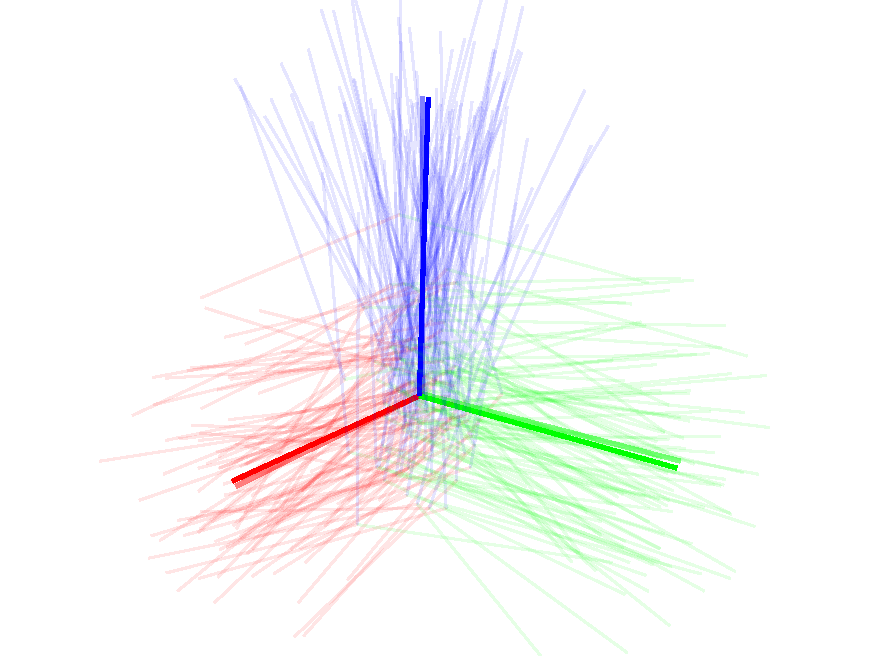
\includegraphics[width=0.75\columnwidth]{figures/mean-pose-example.pdf}
  \captionsetup{type=figure}
  \captionof{figure}{100 randomly drawn poses are shown in thin transparent axes, while the true mean is shown in thick transparent axes. The mean estimated using Algorithm~\ref{alg:iterative-mean-pose} is shown in thick solid axes.}
  \label{fig:mean-pose-example}
  \par
}
The procedure in Algorithm~\ref{alg:iterative-mean-pose} is shown to converge at least linearly if the initial estimate is close enough to the solution \cite{Arsigny2006Bi-invariant.}.
We can also apply the hybrid representation in Section~\ref{sec:hybrid-representation} to simplify the procedure even further.
Figure~\ref{fig:mean-pose-example} shows an example of estimating the mean of a set of randomly drawn poses.
\end{example}

The Gauss-Newton algorithm can approach quadratic convergence rate in some situations.
This is because it computes step lengths by approximating the Hessian of the objective function $f(\ubar{\cX})$ at $\ubar{\hat{\cX}}$ as
\begin{equation}
\begin{split}
  \frac{\partial^2 f(\ubar{\hat{\cX}})}{\partial \ubar{\hat{\cX}} \partial \ubar{\hat{\cX}}\trans} &= \left( \dpar{e(\ubar{\hat{\cX}})}{\ubar{\hat{\cX}}} \right)\trans \left( \dpar{e(\ubar{\hat{\cX}})}{\ubar{\hat{\cX}}} \right) +
  \sum_{i=1}^n e_i(\ubar{\hat{\cX}}_i) \frac{\partial^2 e_i(\ubar{\hat{\cX}}_i)}{\partial \ubar{\hat{\cX}}_i \partial \ubar{\hat{\cX}}_i\trans}\\[1em]
  &= \matA\trans \matA + \matQ \approx \matA\trans \matA.
\end{split}
\end{equation}
This approximation is good if we are near the solution, and the objective function is nearly quadratic.
If the quadratic fit is poor, Gauss-Newton might still estimate decent update directions, but the step lengths may be bad.
This may lead to new estimates that are further away from the minimum, and subsequent divergence.

Since the Gauss-Newton algorithm is not guaranteed to converge because of the Hessian approximation, it is sometimes beneficial to modify the algorithm to be more conservative towards robustness, rather than speed.
One solution is to update the estimate with only a fraction $\alpha$ of the update vector
\begin{equation}
  \ubar{\hat{\cX}}^{t+1} \leftarrow \ubar{\hat{\cX}}^t \oplus \alpha \ubar{\vectau},
\end{equation}
We can find good values for $\alpha$ by performing a \emph{line search} \cite{barfoot2017state}.

Another solution is to apply a \emph{trust region method}, which controls in which region one is willing to trust the quadratic Hessian approximation made by Gauss-Newton.
The \emph{Levenberg-Marquardt} algorithm is an example of such a method, where the normal equations \eqref{eq:ls-normal-equations} are modified by adding a non-negative constant to the diagonal
\begin{equation}
  \left( \matA\trans \matA + \lambda \diag(\matA\trans \matA) \right)\ubar{\vectau} = \matA\trans \vecb.
\end{equation}
When $\lambda = 0$ we obtain Gauss-Newton, while larger $\lambda$ causes larger steps in the steepest descent direction when the gradient is small, and more cautious steps when the gradient is large.
The complete Levenberg-Marquardt method is given in Algorithm~\ref{alg:levenberg-marquardt}.


\begin{algorithm}[H] \label{alg:levenberg-marquardt}
\SetAlgoLined
\DontPrintSemicolon
\KwData{An objective function $f(\ubar{\cX})$ and a good initial state estimate $\ubar{\hat{\cX}}^0$}
\KwResult{An estimate for the states $\ubar{\hat{\cX}}$}
 \;
 $\lambda \leftarrow 10^{-4}$\;
 \;
 \For{$t = 0, 1, \ldots, t^{\text{max}}$}{
  $\matA, \vecb \leftarrow$ Linearise $f(\ubar{\cX})$ at $\ubar{\hat{\cX}}^t$\;
  $\ubar{\vectau} \leftarrow$ Solve the linearised problem $( \matA\trans \matA + \lambda \diag(\matA\trans \matA))\ubar{\vectau} = \matA\trans \vecb$\;
  \;
  \eIf{$f(\ubar{\hat{\cX}}^t \oplus \ubar{\vectau}) < f(\ubar{\hat{\cX}}^t)$}
  {
    Accept update, increase trust region\;
    $\ubar{\hat{\cX}}^{t+1} \leftarrow \ubar{\hat{\cX}}^t \oplus \ubar{\vectau}$\;
    $\lambda \leftarrow \lambda / 10$
  }
  {
    Reject update, reduce trust region\;
    $\ubar{\hat{\cX}}^{t+1} \leftarrow \ubar{\hat{\cX}}^t$\;
    $\lambda \leftarrow \lambda * 10$
  }
  
  \;
  \If{$f(\ubar{\hat{\cX}}^{t+1})$ is very small or $\ubar{\hat{\cX}}^{t+1} \approx \ubar{\hat{\cX}}^t$}{
   $\ubar{\hat{\cX}} \leftarrow \ubar{\hat{\cX}}^{t+1}$\;
   \Return \;
   }
 }
 \caption{The Levenberg-Marquardt algorithm}
\end{algorithm}

\begin{example}[frametitle=Range-based localisation] \label{ex:range-based-localisation}
This example is inspired by an example in \cite{Boyd2017IntroductionSquares}.

{
  \centering
  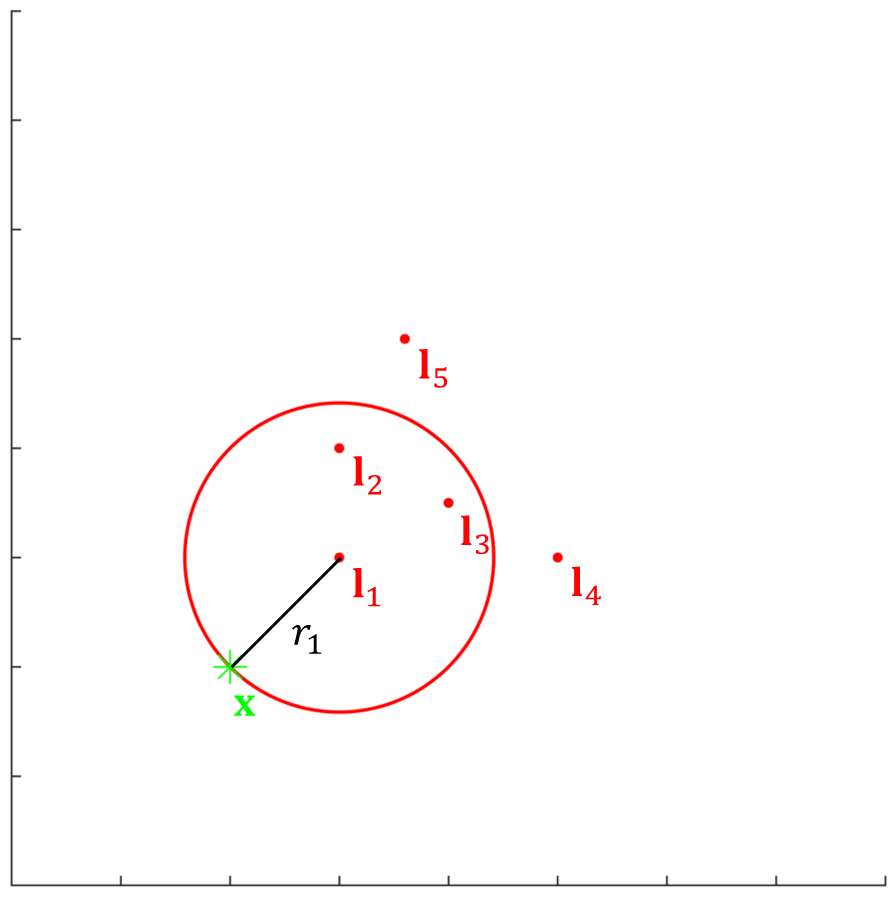
\includegraphics[height=7.5cm]{figures/range-localisation-intro.png}
  \captionsetup{type=figure}
  \captionof{figure}{Range-based localisation example.
  Our true position $\vecx$ is shown in green, while the known landmarks $\{\vecl_1, \ldots, \vecl_5\}$ are shown in red
  The range $r_1$ from $\vecl_1$ to our position is visualised as a red circle around the landmark.
  }
  \label{fig:range-localisation-intro}
  \par
}
We are given a set of ranges $\{r_1, \ldots, r_n\}$ to landmarks with known 2D positions $\{\vecl_1, \ldots, \vecl_n\}$, and we want to estimate our location $\vecx$ that minimises the errors between the predicted range $\norm{\vecx - \vecl_i}$ and the range measurement $r_i$,
\begin{equation}
  e_i(\vecx) = \norm{\vecx - \vecl_i} - r_i.
\end{equation}
This leads to the objective function
\begin{align}
  f(\vecx) &= \sum^n_{i=1} \norm{\norm{\vecx - \vecl_i} - r_i}^2\\
  &= \sum^n_{i=1} \left( \norm{\vecx - \vecl_i} - r_i \right)^2,
\end{align}
which we can solve as the nonlinear least squares problem
\begin{equation}
  \vecx^\ast = \argmin_\vecx \sum^n_{i=1} \left( \norm{\vecx - \vecl_i} - r_i \right)^2.
\end{equation}
We can linearise the error function at the current estimate $\hat{\vecx}$ as
\begin{equation} \label{eq:linearised-range-error}
  e_i(\hat{\vecx} + \delta\vecx) \approx e_i(\hat{\vecx}) + \jac{e_i}{\hat{\vecx}} \delta\vecx
\end{equation}
The Jacobian is given by (see Example~\ref{ex:jacobian-of-norm})
\begin{equation}
  \jac{e_i}{\hat{\vecx}} = \jac{\norm{\hat{\vecx} - \vecl_i}}{\hat{\vecx}} = \frac{(\hat{\vecx} - \vecl_i)\trans}{\norm{\hat{\vecx} - \vecl_i}}.
\end{equation}
Using \eqref{eq:linearised-objective-function}, we get the linearised least squares problem
\begin{align}
  \delta\vecx^\ast &= \argmin_{\delta\vecx} \sum^n_{i=1} \left( \matA_i \delta\vecx - b_i \right)^2\\
  &= \argmin_{\delta\vecx} \norm{\matA \delta\vecx - \vecb}^2,
\end{align}
where
\begin{align}
  \matA_i &= \jac{e_i}{\hat{\vecx}} = \frac{(\hat{\vecx} - \vecl_i)\trans}{\norm{\hat{\vecx} - \vecl_i}}\\
  b_i &= r_i - e_i(\hat{\vecx}) = r_i - \norm{\hat{\vecx} - \vecl_i}
\end{align}
and
\begin{equation}
  \matA =  
  \begin{bmatrix}
    \matA_1\\
    \vdots\\
    \matA_n
  \end{bmatrix}
  \qquad
  \vecb =  
  \begin{bmatrix}
    \vecb_1\\
    \vdots\\
    \vecb_n
  \end{bmatrix}.
\end{equation}
This lets us estimate $\hat{\vecx}$ using Gauss-Newton (Algorithm~\ref{alg:gauss-newton}) or Levenberg-Marquardt (Algorithm~\ref{alg:levenberg-marquardt}).

{
  \centering
  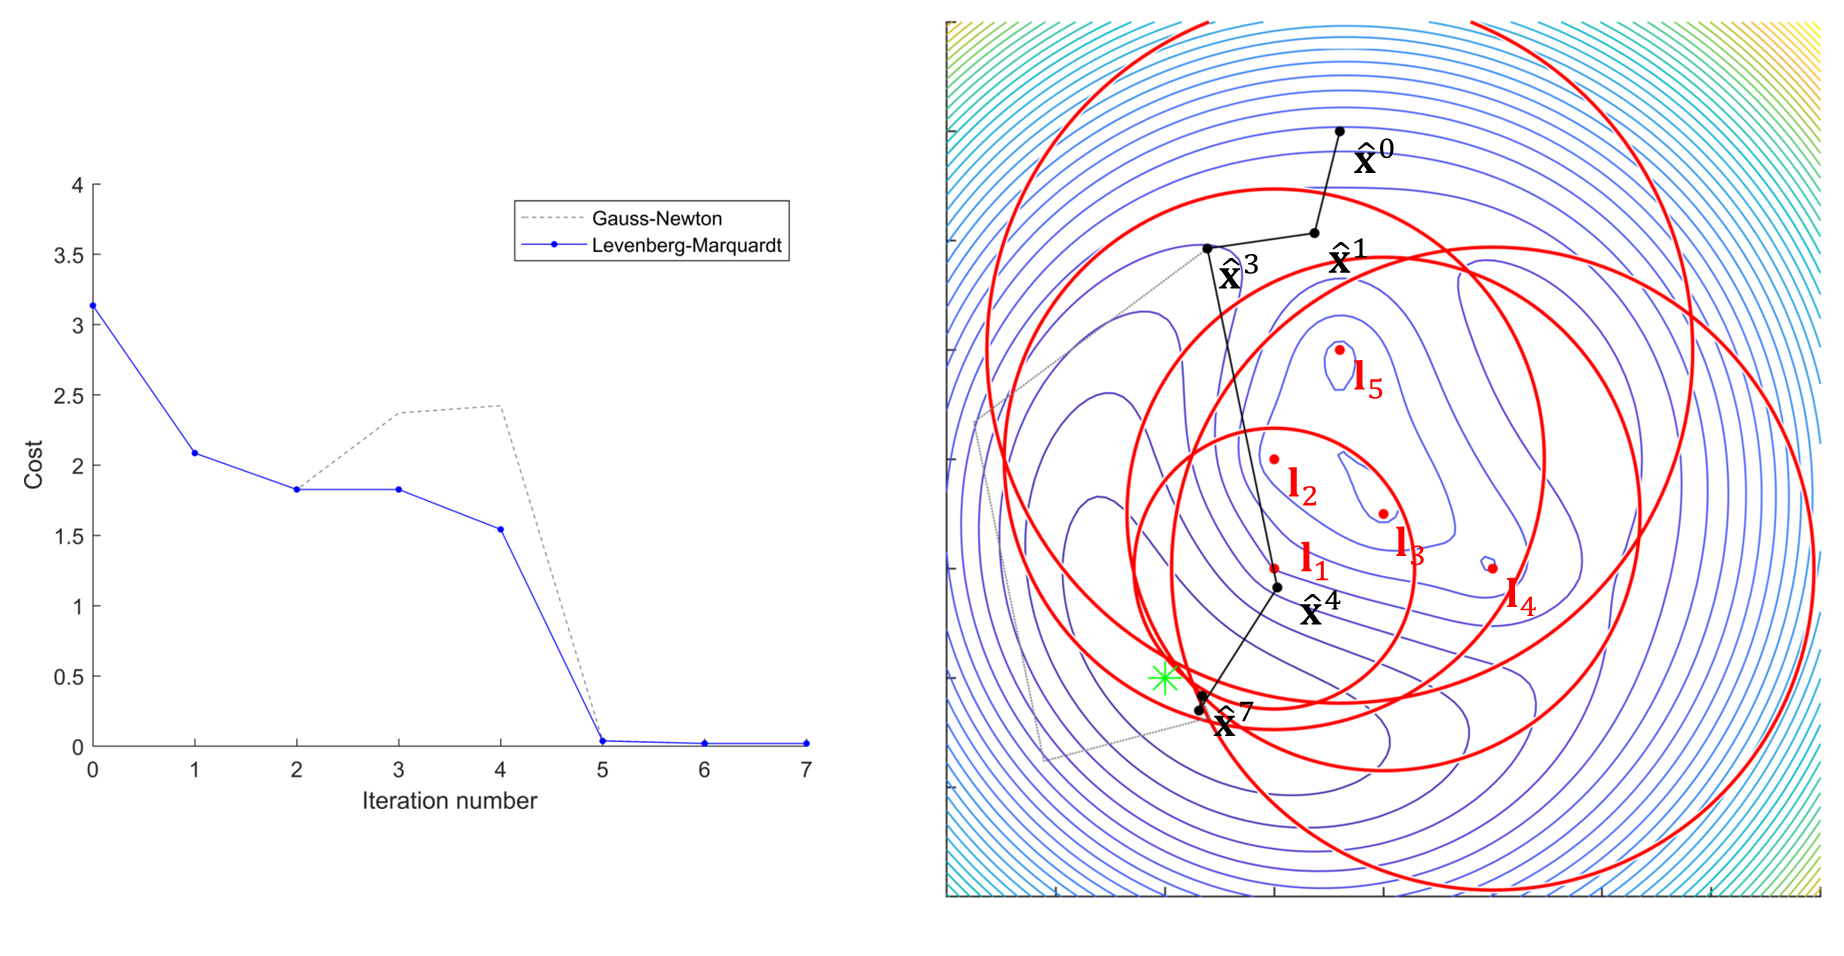
\includegraphics[width=1\columnwidth]{figures/range-localisation-LM-GN.png}
  \captionsetup{type=figure}
  \captionof{figure}{Example of applying Gauss-Newton and Levenberg-Marquardt to the range-based localisation problem.
  The range measurements are shown as red circles around their corresponding landmarks, and the coloured contours visualises the values of objective function at different locations.
  The iteration steps of the Levenberg-Marquardt algorithm are shown in black, while the steps of the Gauss-Newton algorithm are shown in grey.
  To the left we see how the error evolves with iterations for the two algorithms.
  We see that Gauss-Newton performs two steps that increases the error, while Levenberg-Marquardt always reduces the error in each step.
  }
  \label{fig:range-localisation-LM-GN}
  \par
}

Figure~\ref{fig:range-localisation-LM-GN} shows the difference between applying Gauss-Newton and Levenberg-Marquardt.
We see that both methods converge to a solution that minimises the objective function, but Gauss-Newton performs two steps that increases the error.
Figure~\ref{fig:range-localisation-LM-local-minimum} shows that  perturbing the initial estimate slightly results in convergence to an erroneous local minimum.

{
  \centering
  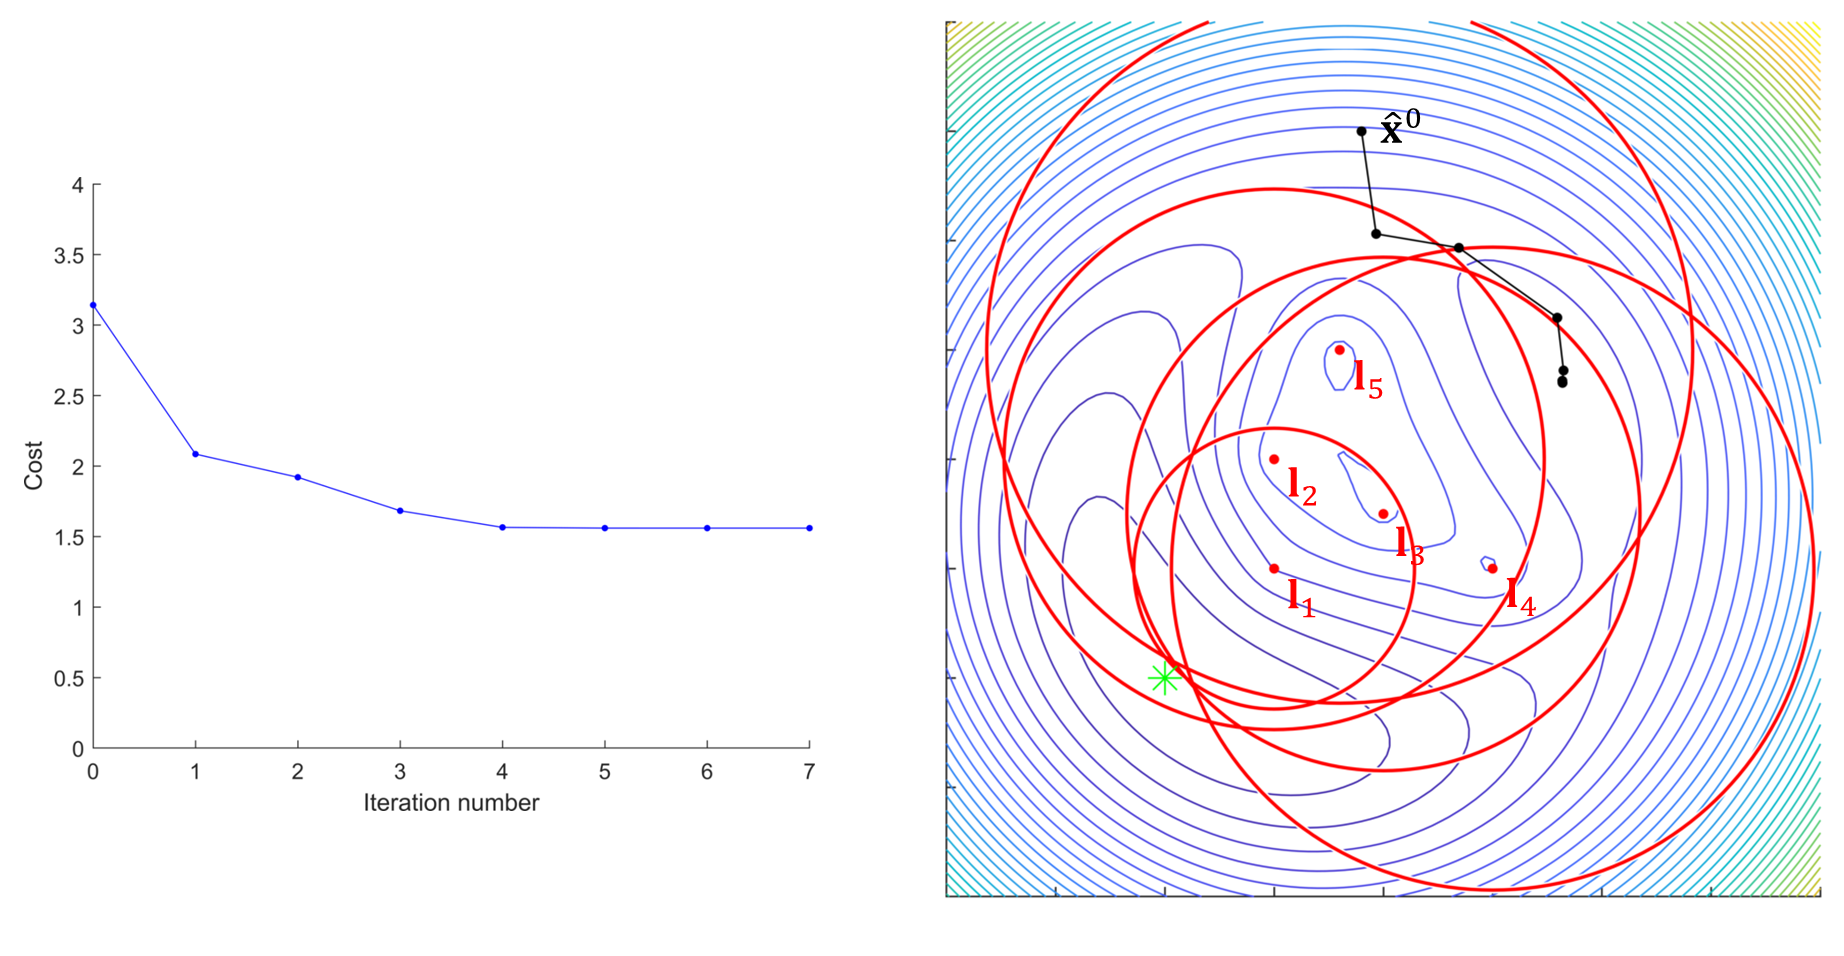
\includegraphics[width=1\columnwidth]{figures/range-localisation-LM-local-minimumpng.png}
  \captionsetup{type=figure}
  \captionof{figure}{The result when perturbing the initial estimate slightly to the right.
  In this situation, Levenberg-Marquardt converges to a local minima.
  Even though Levenberg-Marquardt is guaranteed to converge, it is not guaranteed to converge to the correct solution.
  }
  \label{fig:range-localisation-LM-local-minimum}
  \par
}

\end{example}

\section{Nonlinear MAP inference}
We will now turn to the problem of solving \emph{state estimation problems} based on noisy \emph{measurements}.
Assume that we want to estimate the unknown set of state variables $X$, and that we are given a set of sensor measurements $Z$ that depends upon the true state of $X$.
The most often used estimator for $X$ is the \emph{maximum a posteriori} (MAP) estimate, which maximises the \emph{posterior density} $p(X | Z)$ of the states $X$ given the measurements $Z$,
\begin{align} \label{eq:MAP}
    X^\text{MAP} &= \argmax_X p(X | Z).
\end{align}

Let the states $X$ be represented by the concatenation $\ubar{\cX}$ from \eqref{eq:concatenated-states}, and $Z$ be the set of measurement vectors $Z = \{\vecz_1, \ldots, \vecz_n \}$.
Let $\ubar{\cX}_i$ be the states involved in measurement $\vecz_i$.
Assuming that the measurements are corrupted by zero-mean Gaussian noise, we define the \emph{measurement model} as
\begin{equation}
  \vecz_i = h_i(\ubar{\cX}_i) + \eta_i, \qquad \eta_i \sim \cN(\matr{0}, \matSigma_i),
\end{equation}
where $h_i(\ubar{\cX}_i)$ is the \emph{measurement prediction function}.
We define the \emph{measurement error function} as the difference between the predicted measurement, given the states $\ubar{\cX}_i$, and the measurement $\vecz_i$,
\begin{equation}
  e_i(\ubar{\cX}_i) = h_i(\ubar{\cX}_i) - \vecz_i.
\end{equation}
It can be shown that the MAP estimate for the states $\ubar{\cX}$ given the measurements $Z$ is the solution to the nonlinear least squares problem,
\begin{equation} \label{eq:MAP-nls-problem}
  \ubar{\hat{\cX}}^{\text{MAP}} = \argmin_{\ubar{\cX}} \sum_{i=1}^n \norm{h_i(\ubar{\cX}_i) - \vecz_i}^2_{\matSigma_i},
\end{equation}
where
\begin{equation} \label{eq:mahalanobis-distance}
  \norm{\vece}^2_{\matSigma} \triangleq \vece\trans \matSigma^{-1} \vece = \left( \matSigma^{-1/2} \vece \right)\trans \left( \matSigma^{-1/2} \vece \right) = \norm{\matSigma^{-1/2} \vece}^2,
\end{equation}
is the squared Mahalanobis distance. 
We see from \eqref{eq:mahalanobis-distance} that the measurement errors are weighted according to the measurement uncertainties, so that good measurements will contribute more to the total error than uncertain measurements.
This is called \emph{covariance weighting}, and \eqref{eq:MAP-nls-problem} is therefore sometimes called a \emph{weighted nonlinear least squares} problem.

We can solve \eqref{eq:MAP-nls-problem} by first linearising the measurement prediction functions around the current estimate $\ubar{\hat{\cX}}$,
\begin{equation}
  h_i(\ubar{\cX}_i) = h_i(\ubar{\hat{\cX}}_i \oplus \ubar{\vectau}_i) \approx h_i(\ubar{\hat{\cX}}_i) + \jac{h_i}{\ubar{\hat{\cX}}_i} \ubar{\vectau}_i.
\end{equation}
This leads to the linearised measurement error function
\begin{equation}
  e_i(\ubar{\cX}_i) = e_i(\ubar{\hat{\cX}}_i \oplus \ubar{\vectau}_i) \approx h_i(\ubar{\hat{\cX}}_i) + \jac{h_i}{\ubar{\hat{\cX}}_i} \ubar{\vectau}_i - \vecz_i,
\end{equation}
and the linearised objective function 
\begin{equation} \label{eq:MAP-linearised-objective-function}
\begin{split}
    f(\ubar{\cX}) = f(\ubar{\hat{\cX}} \oplus \ubar{\vectau}) &= \sum^n_{i=1} \norm{e_i(\ubar{\hat{\cX}}_i \oplus \ubar{\vectau}_i)}^2_{\matSigma_i}\\
    &\approx \sum^n_{i=1} \norm{h_i(\ubar{\hat{\cX}}_i) + \jac{h_i}{\ubar{\hat{\cX}}_i} \ubar{\vectau}_i - \vecz_i}^2_{\matSigma_i}\\
    &= \sum^n_{i=1} \norm{\jac{h_i}{\ubar{\hat{\cX}}_i} \ubar{\vectau}_i - (\vecz_i - h_i(\ubar{\hat{\cX}}_i))}^2_{\matSigma_i}\\
    &= \sum^n_{i=1} \norm{\matSigma^{-1/2}_i \jac{h_i}{\ubar{\hat{\cX}}_i} \ubar{\vectau}_i - \matSigma^{-1/2}_i(\vecz_i - h_i(\ubar{\hat{\cX}}_i))}^2\\
    &= \sum^n_{i=1} \norm{\matA_i \ubar{\vectau}_i - \vecb_i}^2\\
    &= \norm{\matA \ubar{\vectau} - \vecb}^2.
\end{split}
\end{equation}
Notice that the weighted Jacobians
\begin{equation}
  \matA_i = \matSigma^{-1/2}_i \jac{h_i}{\ubar{\hat{\cX}}_i},
\end{equation}
and the weighted \emph{measurement prediction errors}
\begin{equation}
  \vecb_i =  \matSigma^{-1/2}_i(\vecz_i - h_i(\ubar{\hat{\cX}}_i)),
\end{equation}
have now undergone a form of \emph{whitening}, that eliminates the units of the measurements.

With the problem on linearised form, we can apply Gauss-Newton (Algorithm~\ref{alg:gauss-newton}) or Levenberg-Marquardt (Algorithm~\ref{alg:levenberg-marquardt}) to compute the MAP estimate $\ubar{\hat{\cX}}$, given a suitable initial estimate $\ubar{\hat{\cX}}^0$.
We can estimate the uncertainty in the MAP estimate by recognising that the Hessian of $f(\ubar{\cX})$ at the solution corresponds to the \emph{information matrix} of the estimate.
Using the Gauss-Newton approximation to the Hessian, we obtain a first order approximation of the true covariance, given by
\begin{equation}
  \matSigma_{\ubar{\hat{\cX}}} = \matLambda_{\ubar{\hat{\cX}}}^{-1} \approx (\matA_{\ubar{\hat{\cX}}}\trans \matA_{\ubar{\hat{\cX}}})^{-1}.
\end{equation}

\begin{example}[frametitle=Range-based localisation with measurement noise] \label{ex:range-based-localisation-noise}
We will revisit the range-based localisation example in Example~\ref{ex:range-based-localisation}, and see how we can apply the framework given in this section to naturally describe the state estimation problem, and solve it in the presence of measurement noise.

We are given a set of noisy range measurements $\{r_1, \ldots, r_n\}$ to landmarks with known 2D positions $\{\vecl_1, \ldots, \vecl_n\}$.
The measurement model is given by
\begin{equation}
  r_i = h_i(\vecx) + \eta_i, \qquad \eta \sim \cN(0, \sigma^2_i),
\end{equation}
where the measurement prediction function is
\begin{equation}
  h_i(\vecx) = \norm{\vecx - \vecl_i}.
\end{equation}
The measurement error is given by
\begin{equation}
  e_i(\vecx) = h_i(\vecx) - r_i = \norm{\vecx - \vecl_i} - r_i,
\end{equation}
leading to the covariance weighted nonlinear least squares problem
\begin{equation} \label{eq:range-MAP-weighted}
  \hat{\vecx}^{\text{MAP}} = \argmin_\vecx \sum^n_{i=1} \frac{1}{\sigma_i} \left( \norm{\vecx - \vecl_i} - r_i \right)^2
\end{equation}
By linearising the problem according to \eqref{eq:linearised-range-error} and \eqref{eq:MAP-linearised-objective-function}, we get the linearised least squares problem
\begin{align} \label{eq:range-MAP-linearised-problem}
  \delta\vecx^\ast &= \argmin_{\delta\vecx} \sum^n_{i=1} \left( \matA_i \delta\vecx - b_i \right)^2\\
  &= \argmin_{\delta\vecx} \norm{\matA \delta\vecx - \vecb}^2,
\end{align}
where
\begin{align}
  \matA_i &= \frac{1}{\sigma_i}\jac{e_i}{\hat{\vecx}} = \frac{1}{\sigma_i}\frac{(\hat{\vecx} - \vecl_i)\trans}{\norm{\hat{\vecx} - \vecl_i}}\\
  b_i &= \frac{1}{\sigma_i}(r_i - e_i(\hat{\vecx})) = \frac{1}{\sigma_i}(r_i - \norm{\hat{\vecx} - \vecl_i}).
\end{align}

Figure~\ref{fig:range-localisation-weighted} illustrates the difference between plain least squares and covariance weighted least squares.
In Figure~\ref{fig:range-localisation-covariance}, we see an illustration of the covariance estimated from the approximation to the Hessian, in the idealised case when all measurements are equal to the expected values.
 
{
  \centering
  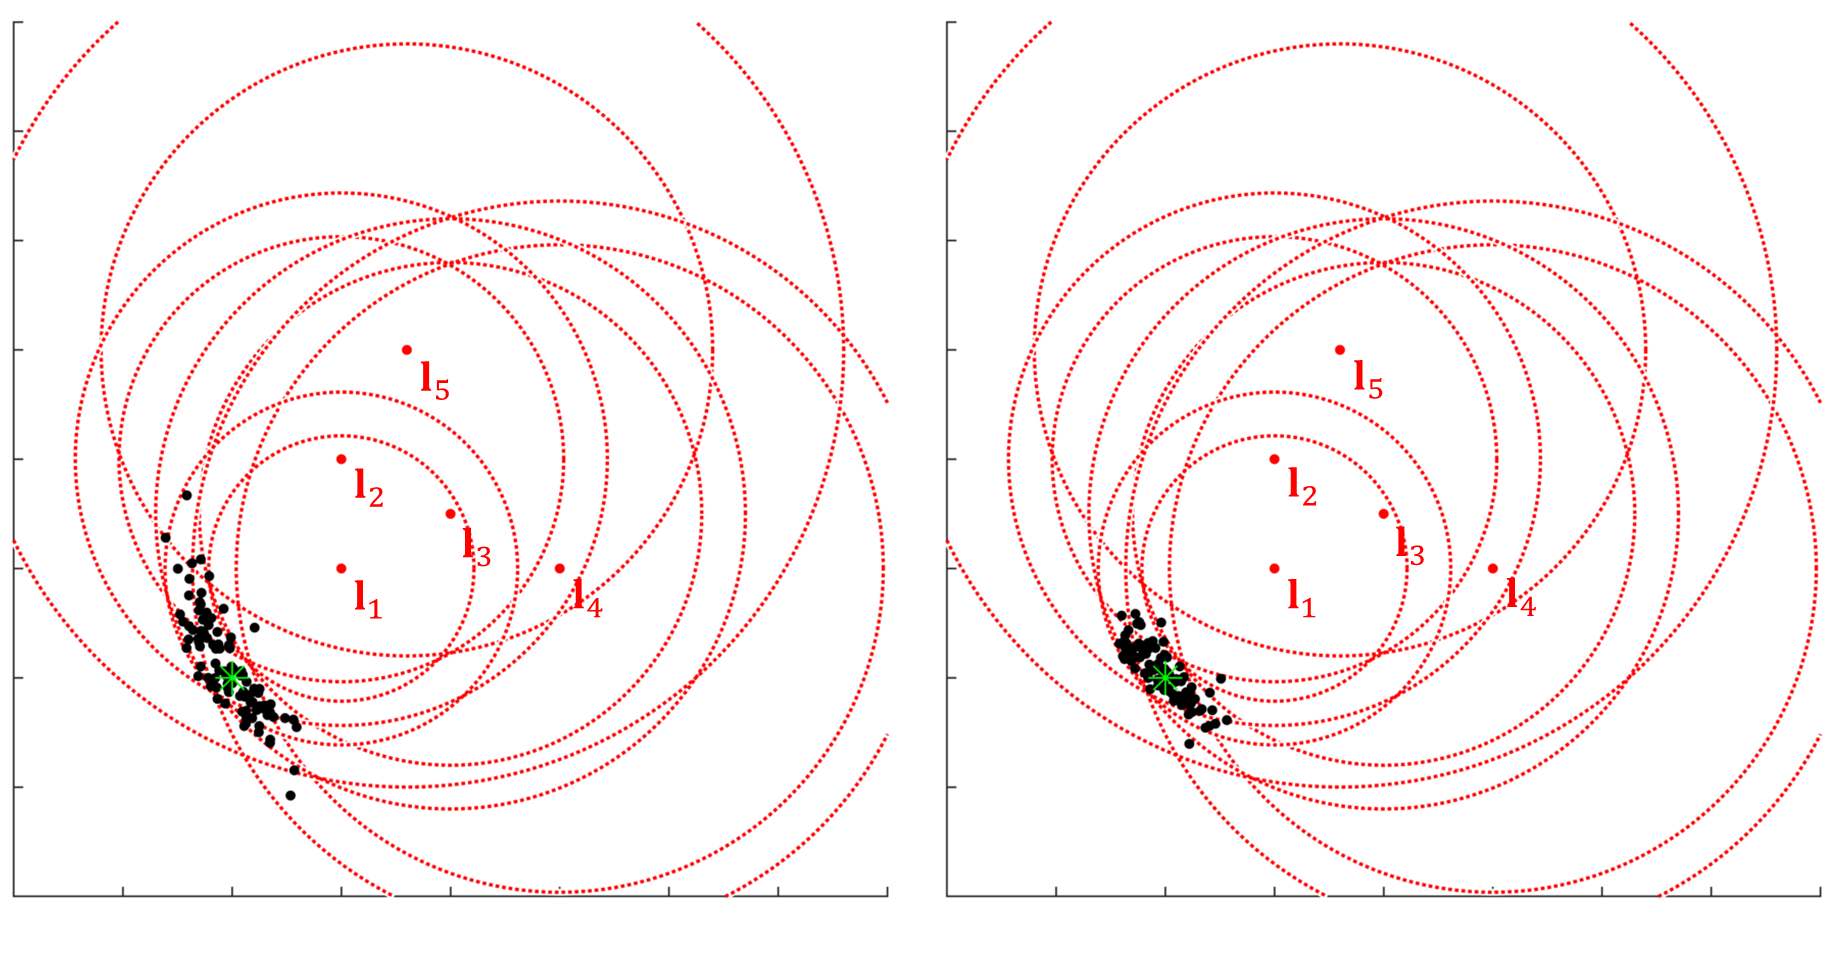
\includegraphics[width=\columnwidth]{figures/range-localisation-weighted.png}
  \captionsetup{type=figure}
  \captionof{figure}{The difference between not taking measurement noise into account, and performing covariance weighting.
  The noise on the range measurements is visualised as $\pm \sigma$ dotted circles around the landmarks.
  In this example, landmark $\vecl_5$ has triple the measurement noise compared to the other landmarks.
  Based on simulating 100 sets of measurements, we see on the left the result of estimating $\vecx$ without taking the noise into account.
  The uncertainty in the results are dominated by the uncertain measurements.
  On right, the same measurements have been used in the covariance weighted scheme in \eqref{eq:range-MAP-weighted}.
  We see that the influence of the noisy measurements have been significantly reduced.
  }
  \label{fig:range-localisation-weighted}
  \par
}

{
  \centering
  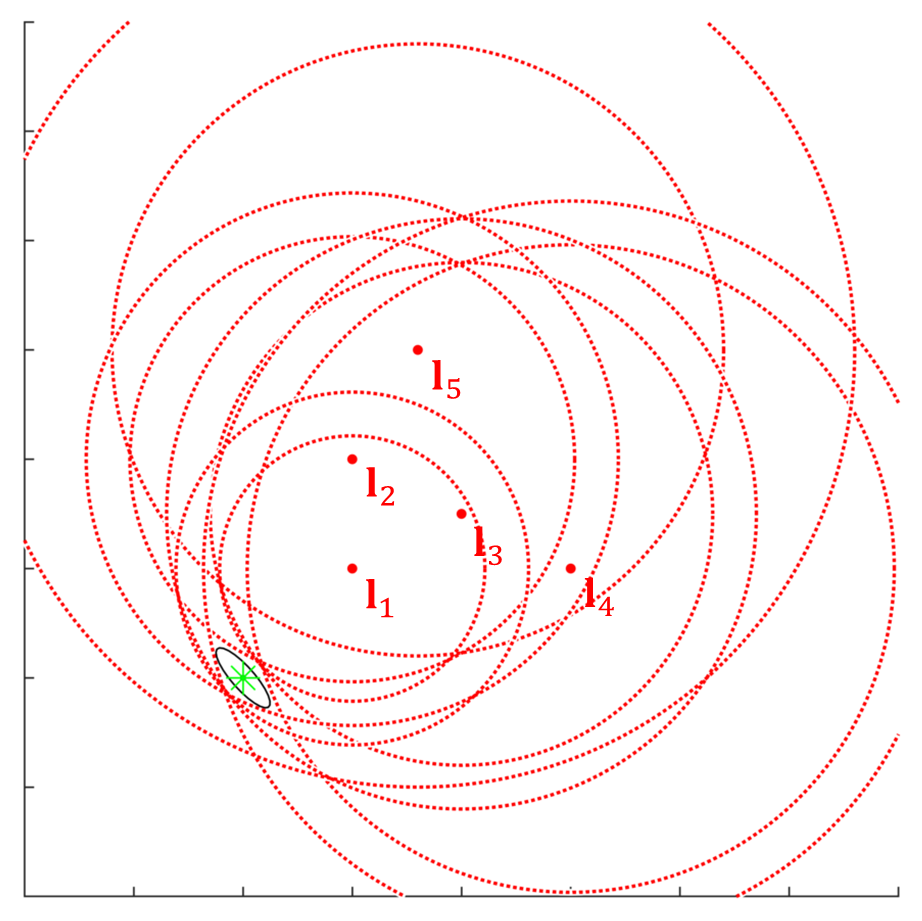
\includegraphics[height=7.5cm]{figures/range-localisation-covariance.png}
  \captionsetup{type=figure}
  \captionof{figure}{The covariance estimated from the approximation of the Hessian at the solution.
  Here, all measurements are set to the mean, to illustrate the connection between the uncertainty in the measurements, visualised as $\pm \sigma$ dotted circles around the landmarks, and the covariance of the estimate, shown as a black ellipse corresponding to the Mahalanobis distance at 1 standard deviation.
  }
  \label{fig:range-localisation-covariance}
  \par
}

\end{example}

The framework for MAP estimation described in this section makes it easy to express estimation problems where we want to find the best estimates for the states $\ubar{\cX}$, given a set of measurements $Z$.
By defining measurement prediction functions $h_i(\ubar{\cX}_i)$ for each measurement $\vecz_i$, and assuming Gaussian measurement noise, we can now obtain the MAP estimate and an estimate for its uncertainty.
This is done by linearising the measurement prediction function, using the tools from Chapter~\ref{ch:jacobians}, and applying the Gauss-Newton method from Algorithm~\ref{alg:gauss-newton} or the Levenberg-Marquardt method in Algorithm~\ref{alg:levenberg-marquardt}.

Notice that we have not assumed that all the measurements have the same type of measurement prediction function.
This means that we also can use this framework to put several different types of constraints on the state variables, such as priors on states, as well as measurements from different types of sensors.
We will in the next section see how we can apply this framework to estimate pose and structure from images.

\begin{example}[frametitle=Range-based localisation with prior]

{
  \centering
  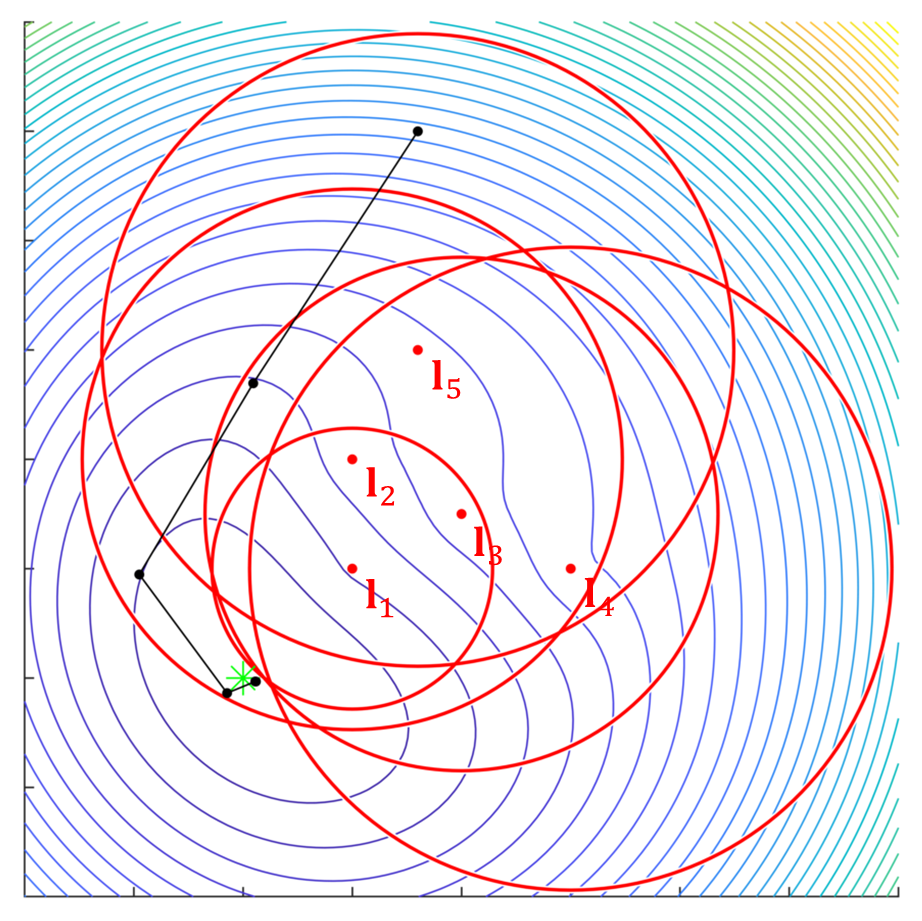
\includegraphics[height=7.5cm]{figures/range-localisation-prior.png}
  \captionsetup{type=figure}
  \captionof{figure}{The result of adding a prior to the problem in \eqref{eq:range-MAP-linearised-problem}.
  The expected value of the prior is set to the true state, and the standard deviation in both directions correspond to the measurement noise for the noisiest landmark $\vecl_5$.
  Compared to Figure~\ref{fig:range-localisation-LM-GN}, we see that the cost function is smoother, with a much better defined global minimium.
  The Gauss-Newton iterations shown in black traverses more directly towards the solution.
  }
  \label{fig:range-localisation-prior}
  \par
}

We can add a prior distribution $\cN(\bar{\vecx}_p, \matSigma_p)$ on our position in the problem in Example~\ref{ex:range-based-localisation-noise}, by adding another constraint on the state $\vecx$.

We can define the ``measurement model'' for the prior distribution as
\begin{equation}
  \matr{0} = h_p(\vecx) + \eta_p, \qquad \eta \sim \cN(\matr{0}, \matSigma_p),
\end{equation}
where the measurement prediction function simply is
\begin{equation}
  h_p(\vecx) = \vecx - \bar{\vecx}_p.
\end{equation}
Since $\jac{h_p}{\hat{\vecx}} = \matI$, we can add the prior constraint by adding the following Jacobian blocks and prediction errors to $\matA$ and $\vecb$ in \eqref{eq:range-MAP-linearised-problem}:
\begin{align}
  \matA_p &= \matSigma_p^{-1/2} \matI = \matSigma_p^{-1/2}\\
  \vecb_p &= \matSigma_p^{-1/2} (\matr{0} - (\vecx - \bar{\vecx}_p)) = \matSigma_p^{-1/2} (\bar{\vecx}_p - \vecx).
\end{align}
Figure~\ref{fig:range-localisation-prior} shows an example of adding a strict prior on $\vecx$. 

\end{example}
